% AUTO-GENERATED by code/figlib.py helpers -- do not edit
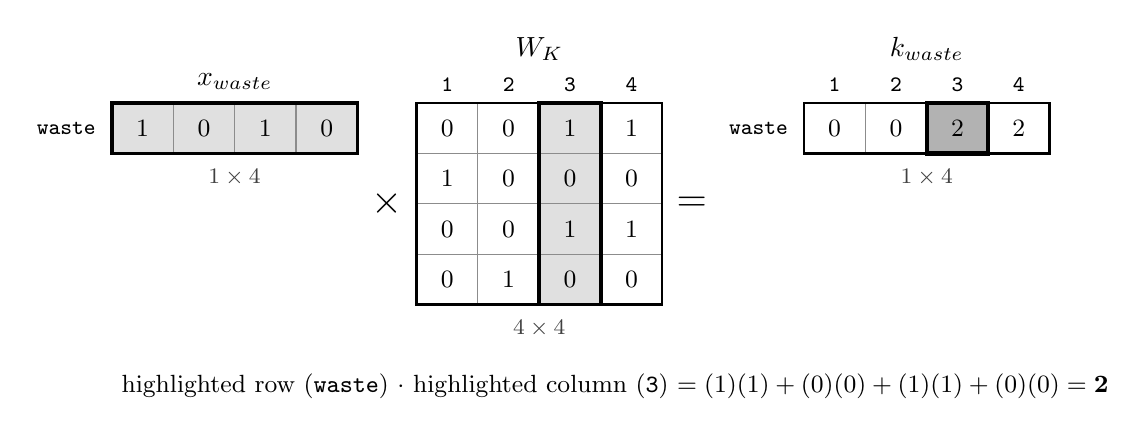
\begin{tikzpicture}
\draw[black!45, fill=black!12] (0.000,0.000) rectangle (0.780,-0.640);
\node[font=\small, text=black] at (0.390,-0.320) {$1$};
\draw[black!45, fill=black!12] (0.780,0.000) rectangle (1.560,-0.640);
\node[font=\small, text=black] at (1.170,-0.320) {$0$};
\draw[black!45, fill=black!12] (1.560,0.000) rectangle (2.340,-0.640);
\node[font=\small, text=black] at (1.950,-0.320) {$1$};
\draw[black!45, fill=black!12] (2.340,0.000) rectangle (3.120,-0.640);
\node[font=\small, text=black] at (2.730,-0.320) {$0$};
\draw[line width=1.4pt] (0.000,0.000) rectangle (3.120,-0.640);
\draw[line width=0.9pt] (0.000,0.000) rectangle (3.120,-0.640);
\node[anchor=east, font=\footnotesize\ttfamily] at (-0.080,-0.320) {waste};
\node[anchor=south, font=\normalsize] at (1.560,0.050) {$\bm{x}_{\text{waste}}$};
\node[anchor=north, font=\footnotesize, text=black!75] at (1.560,-0.720) {$1\times4$};
\draw[black!45, fill=white] (3.870,0.000) rectangle (4.650,-0.640);
\node[font=\small, text=black] at (4.260,-0.320) {$0$};
\draw[black!45, fill=white] (4.650,0.000) rectangle (5.430,-0.640);
\node[font=\small, text=black] at (5.040,-0.320) {$0$};
\draw[black!45, fill=black!12] (5.430,0.000) rectangle (6.210,-0.640);
\node[font=\small, text=black] at (5.820,-0.320) {$1$};
\draw[black!45, fill=white] (6.210,0.000) rectangle (6.990,-0.640);
\node[font=\small, text=black] at (6.600,-0.320) {$1$};
\draw[black!45, fill=white] (3.870,-0.640) rectangle (4.650,-1.279);
\node[font=\small, text=black] at (4.260,-0.959) {$1$};
\draw[black!45, fill=white] (4.650,-0.640) rectangle (5.430,-1.279);
\node[font=\small, text=black] at (5.040,-0.959) {$0$};
\draw[black!45, fill=black!12] (5.430,-0.640) rectangle (6.210,-1.279);
\node[font=\small, text=black] at (5.820,-0.959) {$0$};
\draw[black!45, fill=white] (6.210,-0.640) rectangle (6.990,-1.279);
\node[font=\small, text=black] at (6.600,-0.959) {$0$};
\draw[black!45, fill=white] (3.870,-1.279) rectangle (4.650,-1.919);
\node[font=\small, text=black] at (4.260,-1.599) {$0$};
\draw[black!45, fill=white] (4.650,-1.279) rectangle (5.430,-1.919);
\node[font=\small, text=black] at (5.040,-1.599) {$0$};
\draw[black!45, fill=black!12] (5.430,-1.279) rectangle (6.210,-1.919);
\node[font=\small, text=black] at (5.820,-1.599) {$1$};
\draw[black!45, fill=white] (6.210,-1.279) rectangle (6.990,-1.919);
\node[font=\small, text=black] at (6.600,-1.599) {$1$};
\draw[black!45, fill=white] (3.870,-1.919) rectangle (4.650,-2.558);
\node[font=\small, text=black] at (4.260,-2.239) {$0$};
\draw[black!45, fill=white] (4.650,-1.919) rectangle (5.430,-2.558);
\node[font=\small, text=black] at (5.040,-2.239) {$1$};
\draw[black!45, fill=black!12] (5.430,-1.919) rectangle (6.210,-2.558);
\node[font=\small, text=black] at (5.820,-2.239) {$0$};
\draw[black!45, fill=white] (6.210,-1.919) rectangle (6.990,-2.558);
\node[font=\small, text=black] at (6.600,-2.239) {$0$};
\draw[line width=1.4pt] (5.430,0.000) rectangle (6.210,-2.558);
\draw[line width=0.9pt] (3.870,0.000) rectangle (6.990,-2.558);
\node[anchor=south, font=\footnotesize\ttfamily] at (4.260,0.020) {1};
\node[anchor=south, font=\footnotesize\ttfamily] at (5.040,0.020) {2};
\node[anchor=south, font=\footnotesize\ttfamily] at (5.820,0.020) {3};
\node[anchor=south, font=\footnotesize\ttfamily] at (6.600,0.020) {4};
\node[anchor=south, font=\normalsize] at (5.430,0.420) {$W_K$};
\node[anchor=north, font=\footnotesize, text=black!75] at (5.430,-2.638) {$4\times4$};
\draw[black!45, fill=white] (8.790,0.000) rectangle (9.570,-0.640);
\node[font=\small, text=black] at (9.180,-0.320) {$0$};
\draw[black!45, fill=white] (9.570,0.000) rectangle (10.350,-0.640);
\node[font=\small, text=black] at (9.960,-0.320) {$0$};
\draw[black!45, fill=black!30] (10.350,0.000) rectangle (11.130,-0.640);
\node[font=\small, text=black] at (10.740,-0.320) {$2$};
\draw[black!45, fill=white] (11.130,0.000) rectangle (11.910,-0.640);
\node[font=\small, text=black] at (11.520,-0.320) {$2$};
\draw[line width=1.6pt] (10.350,0.000) rectangle (11.130,-0.640);
\draw[line width=0.9pt] (8.790,0.000) rectangle (11.910,-0.640);
\node[anchor=east, font=\footnotesize\ttfamily] at (8.710,-0.320) {waste};
\node[anchor=south, font=\footnotesize\ttfamily] at (9.180,0.020) {1};
\node[anchor=south, font=\footnotesize\ttfamily] at (9.960,0.020) {2};
\node[anchor=south, font=\footnotesize\ttfamily] at (10.740,0.020) {3};
\node[anchor=south, font=\footnotesize\ttfamily] at (11.520,0.020) {4};
\node[anchor=south, font=\normalsize] at (10.350,0.420) {$\bm{k}_{\text{waste}}$};
\node[anchor=north, font=\footnotesize, text=black!75] at (10.350,-0.720) {$1\times4$};
\node[font=\Large] at (3.495,-1.279) {$\times$};
\node[font=\Large] at (7.365,-1.279) {$=$};
\node[anchor=north west, font=\small, align=left] at (0,-3.308) {highlighted row (\texttt{waste}) $\cdot$ highlighted column (\texttt{3}) $= (1)(1) + (0)(0) + (1)(1) + (0)(0) = \mathbf{2}$};
\end{tikzpicture}
